\section{矩母函数}
\label{sec:weak-mgf}

第~\ref{chap:tail-probabilities}章用矩母函数$M_X(t)=\mathbb{E}[\mathrm{e}^{tX}]$给出尾概率的指数界，并提到它在一定条件下决定分布。它与特征函数只差一个$\mathrm{i}$：把$\mathrm{e}^{\mathrm{i}tX}$换成$\mathrm{e}^{tX}$。可是这一换，被积函数不再有界，$M_X(t)$可能是$+\infty$。本节研究它在哪里有限，有限时能做什么，以及它与特征函数的分工。

\paragraph{有限的范围}
记$D_X=\{t\in\mathbb{R}:M_X(t)<\infty\}$。总有$0\in D_X$。$D_X$是一个区间：若$t_1,t_2\in D_X$，$0<\theta<1$，由$t\mapsto\mathrm{e}^{tx}$的凸性，
\[
 \mathrm{e}^{(\theta t_1+(1-\theta)t_2)x}\leq\theta\,\mathrm{e}^{t_1x}+(1-\theta)\,\mathrm{e}^{t_2x} ,
\]
取期望知$\theta t_1+(1-\theta)t_2\in D_X$。这个区间可以是整条实轴、半直线、有界区间，也可以只有一个点。

几个例子。$\mathcal{N}(0,1)$与$\operatorname{Poisson}(\lambda)$的矩母函数分别是$\mathrm{e}^{t^{2}/2}$与$\exp(\lambda(\mathrm{e}^{t}-1))$，对一切$t$有限。$\operatorname{Exp}(1)$的矩母函数是$1/(1-t)$，$D_X=(-\infty,1)$。标准Cauchy分布的密度只按$x^{-2}$衰减，$t\neq0$时$\mathrm{e}^{tx}$在一侧指数增长，积分发散，$D_X=\{0\}$。$D_X$能否包含$0$的一个邻域，取决于两侧尾部是否都至少按指数衰减。

\paragraph{生成矩}
在$0$的邻域上有限时，矩母函数配得上它的名字。

\begin{theorem}[矩母函数与矩]
\label{thm:weak-mgf-moments}
设存在$t_0>0$，使$M_X(t)<\infty$对$\lvert t\rvert<t_0$成立。则
\begin{enumerate}
 \item 对每个整数$k\geq0$与$0<t<t_0$，
 \begin{equation}
 \mathbb{E}\bigl[\lvert X\rvert^{k}\bigr]\leq\frac{k!}{t^{k}}\bigl(M_X(t)+M_X(-t)\bigr)<\infty ;
 \label{eq:weak-mgf-moment-bound}
 \end{equation}
 \item 对$\lvert t\rvert<t_0$，$M_X(t)=\sum_{k\geq0}t^{k}\,\mathbb{E}[X^{k}]/k!$；
 \item $M_X$在$(-t_0,t_0)$上任意次可导，$M_X^{(k)}(0)=\mathbb{E}[X^{k}]$。
\end{enumerate}
\end{theorem}

\begin{proof}
(1)：对$t>0$，$\mathrm{e}^{t\lvert x\rvert}$的幂级数每一项非负，保留第$k$项，得
\[
 \frac{t^{k}\lvert x\rvert^{k}}{k!}\leq\mathrm{e}^{t\lvert x\rvert}\leq\mathrm{e}^{tx}+\mathrm{e}^{-tx} ,
\]
第二个不等号是因为$\mathrm{e}^{t\lvert x\rvert}$就是$\mathrm{e}^{tx}$与$\mathrm{e}^{-tx}$中较大的一个。代入$X$并取期望即得。

(2)：部分和满足
\[
 \Bigl\lvert\sum_{k=0}^{m}\frac{(tX)^{k}}{k!}\Bigr\rvert\leq\mathrm{e}^{\lvert t\rvert\lvert X\rvert}\leq\mathrm{e}^{tX}+\mathrm{e}^{-tX} ,
\]
右边可积，部分和逐点趋于$\mathrm{e}^{tX}$。由支配收敛定理，期望与求和可以交换。

(3)：由(2)，$M_X$在$(-t_0,t_0)$上是收敛的幂级数，可以逐项求导任意次（可参考\BookChapterRef{chap:univariate-differentiation}{卷一第6章“一元函数的微分”}），$t^{k}$的系数乘以$k!$就是$k$阶导数在$0$处的值。
\end{proof}

这回答了第~\ref{chap:tail-probabilities}章留下的问题：逐项取期望的依据是支配收敛定理，控制函数是$\mathrm{e}^{tX}+\mathrm{e}^{-tX}$，它的可积性正来自$0$两侧的有限性。例如$X\sim\operatorname{Exp}(1)$，$1/(1-t)=\sum_{k\geq0}t^{k}$对$\lvert t\rvert<1$成立，比较系数得
\[
 \mathbb{E}[X^{k}]=k!,\qquad k=0,1,2,\dots .
\]

\paragraph{识别分布}
矩母函数在$0$的邻域上相同，能否推出分布相同？借助特征函数可以证明。思路是：矩母函数相同推出各阶矩相同；指数矩有限又使特征函数在每一点附近都能用Taylor级数表示，于是可以从原点出发，一段一段地推出两个特征函数处处相同。

\begin{theorem}[矩母函数确定分布]
\label{thm:weak-mgf-uniqueness}
设存在$t_0>0$，使$M_X(t)=M_Y(t)<\infty$对$\lvert t\rvert<t_0$成立，则$P_X=P_Y$。
\end{theorem}

\begin{proof}
取$0<r<t_0$。先证明：对每个$s\in\mathbb{R}$与$\lvert h\rvert\leq r$，
\begin{equation}
 \phi_X(s+h)=\sum_{k\geq0}\frac{\phi_X^{(k)}(s)}{k!}h^{k} .
 \label{eq:weak-cf-taylor-series}
\end{equation}
由定理~\ref{thm:weak-mgf-moments}，各阶矩有限，式~\eqref{eq:weak-cf-derivatives}给出各阶导数$\phi_X^{(k)}(s)$的期望表示。在引理~\ref{lem:weak-exp-remainder}中取$x=hX$，乘以$\mathrm{e}^{\mathrm{i}sX}$并取期望，
\[
 \Bigl\lvert\phi_X(s+h)-\sum_{k=0}^{m}\frac{\phi_X^{(k)}(s)}{k!}h^{k}\Bigr\rvert\leq\frac{\mathbb{E}\bigl[\lvert hX\rvert^{m+1}\bigr]}{(m+1)!} .
\]
由单调收敛定理，
\[
 \sum_{m\geq0}\frac{\mathbb{E}[\lvert hX\rvert^{m}]}{m!}=\mathbb{E}\bigl[\mathrm{e}^{\lvert h\rvert\lvert X\rvert}\bigr]\leq M_X(r)+M_X(-r)<\infty ,
\]
级数收敛，通项趋于零，于是式~\eqref{eq:weak-cf-taylor-series}成立。对$Y$同样成立。

由定理~\ref{thm:weak-mgf-moments}(3)，$X$与$Y$的各阶矩相同，由式~\eqref{eq:weak-cf-derivatives}，$\phi_X$与$\phi_Y$在原点的各阶导数相同。在式~\eqref{eq:weak-cf-taylor-series}中取$s=0$，得$\phi_X=\phi_Y$在$[-r,r]$上成立。

再逐段推广。设已知$\phi_X=\phi_Y$在开区间$(-a,a)$上成立，$a\geq r$。取$s=a-r/2$，它在$(-a,a)$内部，两个函数在$s$的一个邻域上相同，所以各阶导数在$s$处相同。由式~\eqref{eq:weak-cf-taylor-series}，两个函数在$[s-r,s+r]$上相同，右端点$a+r/2$超过了$a$。对$-s$作同样的论证。于是$\phi_X=\phi_Y$在$(-a-r/2,a+r/2)$上成立，重复下去覆盖整条实轴。由定理~\ref{thm:weak-cf-uniqueness}，$P_X=P_Y$。
\end{proof}

特征函数在这里仍是识别的工具，矩母函数的作用是保证特征函数可以由原点处的各阶导数完全决定。类似地可以证明：若$M_{X_n}(t)\to M_X(t)$对$0$的某个邻域内的每个$t$成立，且右边有限，则$X_n\xrightarrow{\mathrm{d}}X$；证明要先由矩母函数的一致有界得到胎紧，再用第~\ref{sec:weak-integral-limits}节的方法识别极限，可查阅~\scite{math-kallenberg2021probability}。独立和的矩母函数也是各项矩母函数之积，只要各项在相应的$t$处有限，证明与定理~\ref{thm:weak-cf-independent}相同。

\paragraph{对数正态分布}
所有矩都有限，是否就保证矩母函数在$0$的邻域有限？对数正态分布给出否定的回答。设$Z\sim\mathcal{N}(0,1)$，$Y=\mathrm{e}^{Z}$。由高斯的矩母函数，各阶矩都有限：
\[
 \mathbb{E}[Y^{k}]=\mathbb{E}\bigl[\mathrm{e}^{kZ}\bigr]=\mathrm{e}^{k^{2}/2},\qquad k=0,1,2,\dots .
\]
可是对任意$t>0$，
\[
 M_Y(t)=\int_{-\infty}^{\infty}\frac{1}{\sqrt{2\pi}}\exp\Bigl(t\,\mathrm{e}^{z}-\frac{z^{2}}{2}\Bigr)\,\mathrm{d}z=+\infty ,
\]
因为$z\to\infty$时$t\,\mathrm{e}^{z}$比$z^{2}/2$增长得快，被积函数趋于无穷。$t\leq0$时$\mathrm{e}^{tY}\leq1$，$M_Y(t)$有限。所以$D_Y=(-\infty,0]$，不含$0$的邻域，定理~\ref{thm:weak-mgf-uniqueness}不能用。

这不只是证明方法的缺陷：确实存在另一个分布与$Y$有完全相同的各阶矩。记$f$为$Y$的密度，对$\lvert a\rvert\leq1$令
\[
 f_a(y)=f(y)\bigl(1+a\sin(2\pi\ln y)\bigr),\qquad y>0 .
\]
$f_a\geq0$。下面验证它的各阶矩与$f$相同，$k=0$时即得$f_a$是密度。

只需证明对每个$k\geq0$，
\[
 \int_0^{\infty}y^{k}f(y)\sin(2\pi\ln y)\,\mathrm{d}y=0 .
\]
用$y=\mathrm{e}^{z}$换元，左边等于$\mathbb{E}[\mathrm{e}^{kZ}\sin(2\pi Z)]$。对指数配方，$kz-z^{2}/2=k^{2}/2-(z-k)^{2}/2$，所以
\[
 \mathrm{e}^{kz}\varphi(z)=\mathrm{e}^{k^{2}/2}\varphi(z-k) ,
\]
于是
\[
 \mathbb{E}\bigl[\mathrm{e}^{kZ}\sin(2\pi Z)\bigr]=\mathrm{e}^{k^{2}/2}\,\mathbb{E}\bigl[\sin\bigl(2\pi(Z+k)\bigr)\bigr]=\mathrm{e}^{k^{2}/2}\,\mathbb{E}\bigl[\sin(2\pi Z)\bigr]=0 .
\]
第二个等号用了$k$是整数、正弦的周期是$2\pi$；最后一个等号是因为$\sin(2\pi z)\varphi(z)$是奇函数。

$a\neq0$时$f_a$与$f$是不同的密度，各阶矩却全部相同，图~\ref{fig:weak-lognormal}画出了$a=1/2$的情形。这就是第~\ref{chap:random-variable-moments}章提到的情形：尾部较重时，全部矩也不能确定分布。两者的特征函数当然不同，由定理~\ref{thm:weak-cf-uniqueness}，这是必然的。

\begin{BookInlineFigure}
 \centering
 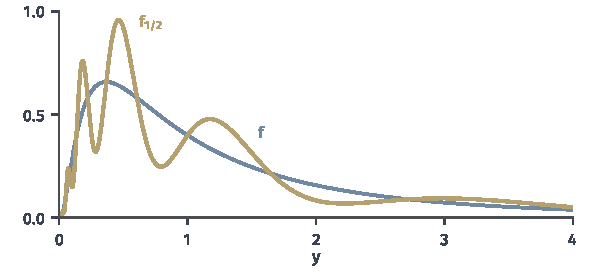
\includegraphics[width=100mm]{figures/07-probability/03-probability-limits/matplotlib/weak-lognormal/figure.pdf}
 \caption{各阶矩相同的两个密度。蓝线为对数正态密度$f$，黄线为$f_{1/2}(y)=f(y)(1+\frac12\sin(2\pi\ln y))$。脚本用数值积分核对了二者的前四阶矩都等于$\mathrm{e}^{k^2/2}$。}
 \label{fig:weak-lognormal}
\end{BookInlineFigure}

\paragraph{两种表示的分工}
下表比较两种变换。特征函数总存在，识别分布与刻画弱收敛都不需要附加条件；矩母函数是实值的，便于计算矩和尾部的指数界，但只有在$0$的邻域上有限时才能用于识别。下一章证明中心极限定理时只假定方差有限，矩母函数可能处处无穷（例如$t$分布），所以证明用特征函数，不以矩母函数存在作为前提。

\begin{BookInlineTable}
 \centering
 \caption{特征函数与矩母函数}
 \label{tab:weak-cf-mgf}
 \begin{tabular}{@{}lll@{}}
 \toprule
 & 特征函数$\phi_X(t)$ & 矩母函数$M_X(t)$\\
 \midrule
 存在范围 & 一切$t$，模不超过$1$ & 区间$D_X$，可能只有$\{0\}$\\
 读出矩 & $k$阶矩有限时求$k$次导 & $0$的邻域有限时全部矩\\
 识别分布 & 无条件 & 需$0$的邻域有限\\
 收敛判据 & 连续性定理 & 需$0$的邻域上收敛\\
 独立和 & 乘积 & 乘积（在有限处）\\
 \bottomrule
 \end{tabular}
\end{BookInlineTable}
